\chapter{Projekt systemu i struktura rozwiązania}
\label{cha:projekt-systemu}

\section{Modelowanie systemu}
\label{sec:modelowanie-systemu}

Modelowanie systemu stanowi jeden z kluczowych etapów projektowania gry \emph{Godmist} z perspektywy inżynierii oprogramowania. Ze względu na złożoność projektowanego rozwiązania konieczne jest opisanie zarówno zachowania systemu z punktu widzenia użytkownika, jak i jego struktury wewnętrznej. W tym celu zastosowano wybrane diagramy języka UML, które pozwalają uporządkować zależności pomiędzy poszczególnymi elementami projektu oraz ułatwiają późniejszą implementację.

W przypadku systemu \emph{Godmist} modelowanie obejmuje kilka wzajemnie uzupełniających się perspektyw. Pierwszą z nich jest perspektywa funkcjonalna, pokazująca, jakie działania może wykonywać użytkownik oraz jakie funkcje system powinien udostępniać. Drugą perspektywą jest opis przebiegu wybranych procesów, takich jak walka, eksploracja lochu, crafting lub zapis gry. Trzecią perspektywę stanowi model zachowania poszczególnych obiektów, na przykład postaci lub misji, których stan zmienia się w czasie rozgrywki.

Zastosowanie diagramów UML w projekcie pozwala przedstawić logikę działania systemu w sposób bardziej formalny i czytelny. Dzięki temu możliwe jest nie tylko lepsze zrozumienie zależności pomiędzy modułami gry, ale również weryfikacja spójności założeń jeszcze przed pełną implementacją. W przypadku gry obejmującej wiele mechanik, takich jak rozwój postaci, walka turowa, eksploracja proceduralnych lochów, zarządzanie ekwipunkiem, interakcje z NPC oraz system misji, etap modelowania jest szczególnie istotny.

W kolejnych podsekcjach przedstawione zostaną wybrane modele systemu: diagram przypadków użycia, scenariusze przypadków użycia, diagramy aktywności, diagramy sekwencji oraz diagramy stanów.

\subsection{Diagramy przypadków użycia}

Ze względu na szeroki zakres funkcjonalny systemu \emph{Godmist} oraz dużą liczbę relacji pomiędzy przypadkami użycia, zrezygnowano z przedstawiania wszystkich funkcji w postaci jednego zbiorczego diagramu. Zamiast tego zastosowano podział na trzy mniejsze diagramy przypadków użycia, odpowiadające głównym obszarom logiki systemu. Takie podejście pozwala zachować czytelność modeli, a jednocześnie nie powoduje utraty istotnych zależności pomiędzy funkcjami.

Pierwszy diagram obejmuje obsługę sesji gry, eksplorację oraz walkę. Drugi koncentruje się na zarządzaniu postacią i ekwipunkiem, natomiast trzeci przedstawia funkcje związane z interakcjami z NPC, handlem, craftingiem oraz obsługą questów. Łącznie trzy diagramy tworzą spójny obraz funkcjonalny projektowanego systemu z perspektywy głównego aktora, którym jest gracz.

\begin{figure}[H]
    \centering
    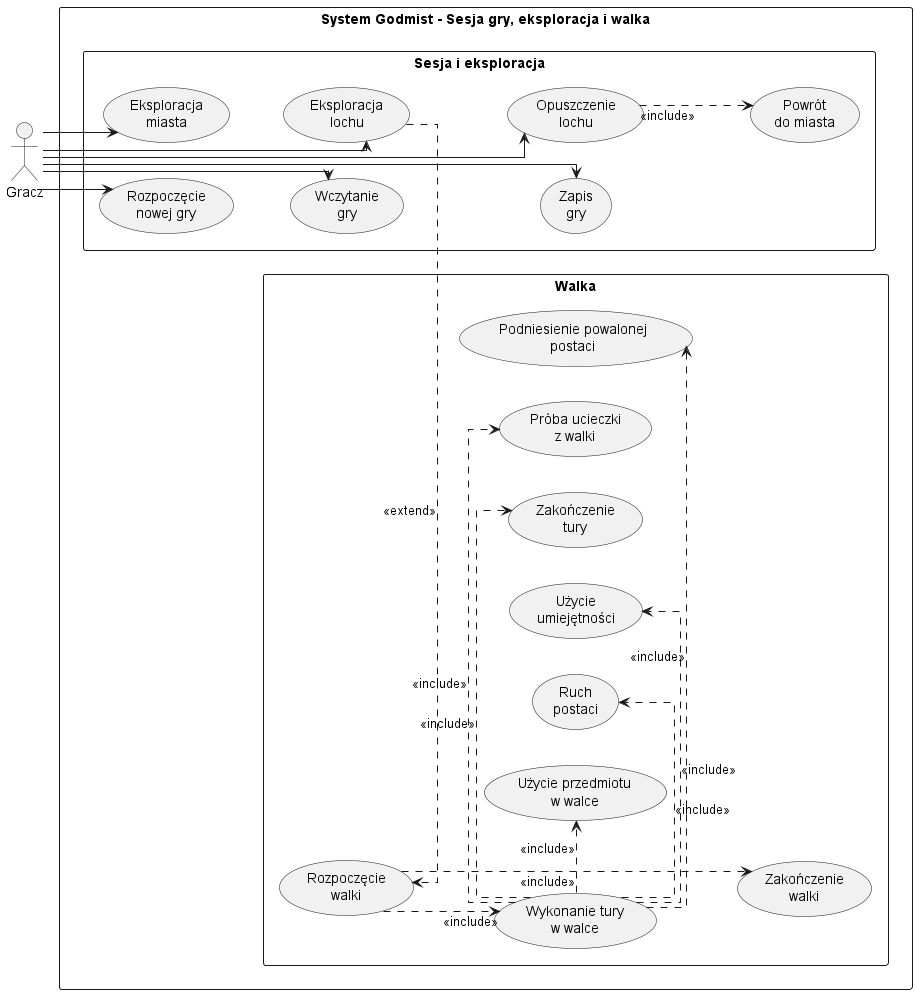
\includegraphics[width=\textwidth,height=0.78\textheight,keepaspectratio]{figures/uml/uc1.png}
    \caption{Diagram przypadków użycia dla sesji gry, eksploracji i walki.}
    \label{fig:use-case-session-exploration-combat}
    \wsizsource{Opracowanie własne}
\end{figure}

Pierwszy diagram przedstawia funkcje związane z rozpoczęciem i obsługą sesji gry, eksploracją miasta i lochu oraz przejściem do systemu walki. Szczególnie istotna jest tu relacja \textit{extend} pomiędzy eksploracją lochu a rozpoczęciem walki, ponieważ pokazuje ona, że walka stanowi zdarzenie uruchamiane w określonym kontekście eksploracji. Diagram obejmuje również podstawowe działania wykonywane w trakcie starcia oraz zakończenie walki i powrót z lochu do miasta.

\begin{figure}[H]
    \centering
    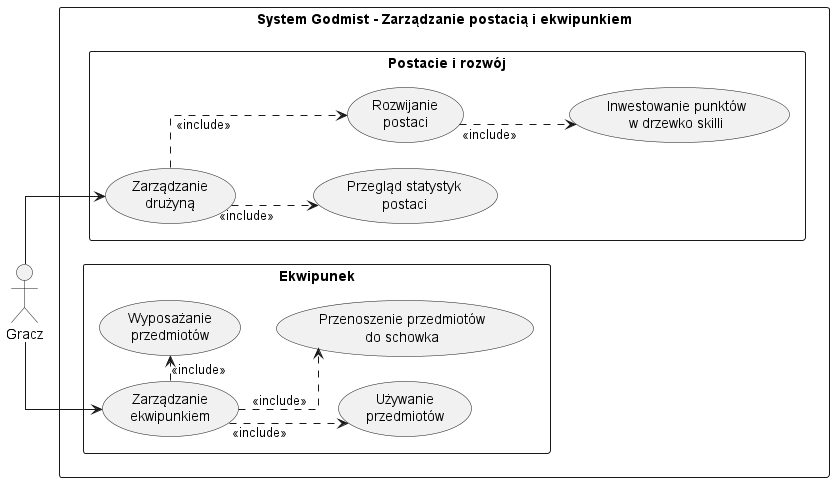
\includegraphics[width=0.9\textwidth,height=0.68\textheight,keepaspectratio]{figures/uml/uc2.png}
    \caption{Diagram przypadków użycia dla zarządzania postacią i ekwipunkiem.}
    \label{fig:use-case-character-inventory}
    \wsizsource{Opracowanie własne}
\end{figure}

Drugi diagram koncentruje się na funkcjach związanych z zarządzaniem drużyną, rozwojem postaci oraz obsługą ekwipunku. Pokazano na nim zależności pomiędzy przeglądem statystyk, rozwijaniem postaci i inwestowaniem punktów w drzewka skilli, a także podstawowe operacje wykonywane na przedmiotach. Diagram ten przedstawia obszar systemu odpowiedzialny za rozwój drużyny oraz organizację zasobów gracza poza bezpośrednim przebiegiem walki.

\begin{figure}[H]
    \centering
    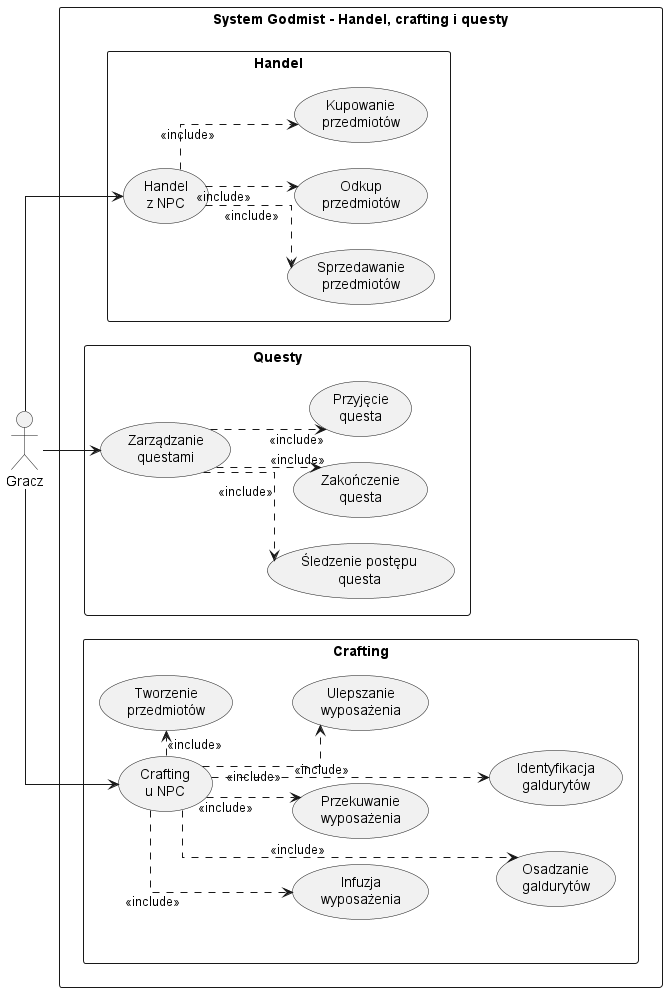
\includegraphics[width=\textwidth,height=0.78\textheight,keepaspectratio]{figures/uml/uc3.png}
    \caption{Diagram przypadków użycia dla handlu, craftingu i questów.}
    \label{fig:use-case-npc-services}
    \wsizsource{Opracowanie własne}
\end{figure}

Trzeci diagram obejmuje funkcje realizowane głównie w interakcji z postaciami niezależnymi, a więc handel, crafting oraz zarządzanie questami. Zostały na nim przedstawione zarówno podstawowe operacje handlowe, jak i bardziej rozbudowane działania związane z ulepszaniem wyposażenia, infuzją oraz obsługą galdurytów. Ujęcie questów w tym samym diagramie wynika z ich silnego powiązania z interakcjami z NPC oraz miejskim zapleczem rozgrywki.
\subsection{Scenariusze przypadków użycia}
\label{subsec:scenariusze-przypadkow-uzycia}

W niniejszym podrozdziale przedstawiono dwa przykładowe scenariusze przypadków użycia dla systemu \emph{Godmist}. Wybrane scenariusze obejmują jeden przypadek związany bezpośrednio z rozgrywką oraz jeden przypadek o charakterze systemowym. Pozwala to pokazać zarówno logikę mechanik gry, jak i obsługę trwałości danych.

\subsubsection*{Scenariusz przypadku użycia: Rozpoczęcie walki}

\textbf{Nazwa przypadku użycia:} Rozpoczęcie walki

\textbf{Aktor główny:} Gracz

\textbf{Cel:} Rozpoczęcie starcia pomiędzy drużyną gracza a przeciwnikami w wyniku eksploracji, interakcji skryptowej lub dialogu.

\textbf{Warunki wstępne:}
\begin{itemize}
    \item gra znajduje się w stanie aktywnej eksploracji miasta lub lochu,
    \item na mapie istnieje grupa jednostek lub zdarzenie mogące wywołać walkę,
    \item stan gry pozwala na przejście do trybu walki.
\end{itemize}

\textbf{Warunki końcowe:}
\begin{itemize}
    \item zostaje utworzona aktywna sesja walki,
    \item uczestnicy walki zostają przypisani do odpowiednich drużyn i relacji,
    \item zostaje wyznaczona kolejność tur,
    \item interfejs użytkownika przechodzi do trybu walki.
\end{itemize}

\textbf{Przebieg główny:}
\begin{enumerate}
    \item Gracz porusza drużyną po mapie lub podejmuje interakcję prowadzącą do starcia.
    \item System wykrywa spełnienie warunku rozpoczęcia walki.
    \item System identyfikuje jednostki biorące udział w starciu.
    \item System wyznacza obszar walki na podstawie miejsca kontaktu i aktualnej mapy.
    \item System tworzy instancję sesji walki.
    \item System przekształca uczestników zdarzenia w jednostki bojowe wraz z ich bieżącym stanem.
    \item System przypisuje uczestników do odpowiednich drużyn oraz określa relacje pomiędzy nimi.
    \item System inicjalizuje parametry walki, w tym pozycje jednostek, aktualne punkty akcji i zasoby.
    \item System wyznacza kolejność tur zgodnie z obowiązującymi regułami.
    \item System przełącza interfejs użytkownika do trybu walki.
    \item System przekazuje sterowanie pierwszej jednostce w kolejności tury.
\end{enumerate}

\textbf{Przebiegi alternatywne:}
\begin{itemize}
    \item Jeżeli walka została wywołana przez dialog, system rozpoczyna starcie po zakończeniu wybranej kwestii dialogowej.
    \item Jeżeli na planszy występują neutralne lub sojusznicze jednostki niezależne, system może dodać je do walki zgodnie z relacjami do drużyn.
    \item Jeżeli starcie przestaje być zasadne jeszcze przed właściwą inicjalizacją, system nie tworzy sesji walki i pozostaje w trybie eksploracji.
\end{itemize}

\textbf{Uwagi:}
\begin{itemize}
    \item rozpoczęcie walki nie przenosi gracza do oddzielnej mapy, lecz wykorzystuje tę samą przestrzeń podzieloną na pola,
    \item pole walki zależy od aktualnego otoczenia, na przykład korytarza, pomieszczenia lub otwartego terenu.
\end{itemize}

\subsubsection*{Scenariusz przypadku użycia: Zapis gry}

\textbf{Nazwa przypadku użycia:} Zapis gry

\textbf{Aktor główny:} Gracz

\textbf{Cel:} Utrwalenie aktualnego stanu gry w pliku zapisu, tak aby można było go później odtworzyć.

\textbf{Warunki wstępne:}
\begin{itemize}
    \item gra znajduje się w stanie, w którym zapis jest dozwolony,
    \item istnieje aktywna kampania lub aktywny stan rozgrywki,
    \item system posiada dostęp do lokalizacji przeznaczonej na pliki zapisu.
\end{itemize}

\textbf{Warunki końcowe:}
\begin{itemize}
    \item aktualny stan gry zostaje zapisany w nowym lub zaktualizowanym wpisie listy zapisów,
    \item metadane zapisu zostają zaktualizowane,
    \item użytkownik otrzymuje informację o powodzeniu lub niepowodzeniu operacji.
\end{itemize}

\textbf{Przebieg główny:}
\begin{enumerate}
    \item Gracz wybiera opcję zapisu gry z poziomu interfejsu systemowego.
    \item System weryfikuje, czy aktualny stan gry pozwala na wykonanie zapisu.
    \item System pobiera bieżący stan postaci, świata, questów, lochów, NPC, schowka i innych istotnych elementów rozgrywki.
    \item System przekształca dane runtime do struktur przeznaczonych do serializacji.
    \item System buduje kompletny obiekt danych zapisu gry.
    \item System serializuje dane do formatu JSON.
    \item System zapisuje dane do pliku.
    \item System aktualizuje metadane zapisu, takie jak data, nazwa lub identyfikator zapisu.
    \item System odświeża listę dostępnych zapisów.
    \item System informuje gracza o poprawnym zakończeniu operacji.
\end{enumerate}

\textbf{Przebiegi alternatywne:}
\begin{itemize}
    \item Jeżeli zapis gry jest niedozwolony w aktualnym stanie, system przerywa operację i wyświetla odpowiedni komunikat.
    \item Jeżeli podczas serializacji lub zapisu pliku wystąpi błąd, system zgłasza niepowodzenie operacji i nie nadpisuje poprawnych wcześniejszych zapisów.
    \item Jeżeli zapis wykonywany jest automatycznie, system pomija część interakcji użytkownika i zapisuje stan zgodnie z regułami autosave.
\end{itemize}

\textbf{Uwagi:}
\begin{itemize}
    \item zapis gry obejmuje zarówno stan postaci i ich wyposażenia, jak i postęp questów, stan świata, lochów oraz informacje o usługach i ofertach NPC,
    \item model zapisu oparty jest na plikach JSON i nie wykorzystuje relacyjnej bazy danych.
\end{itemize}

\subsection{Diagramy aktywności}

\begin{figure}[H]
    \centering
    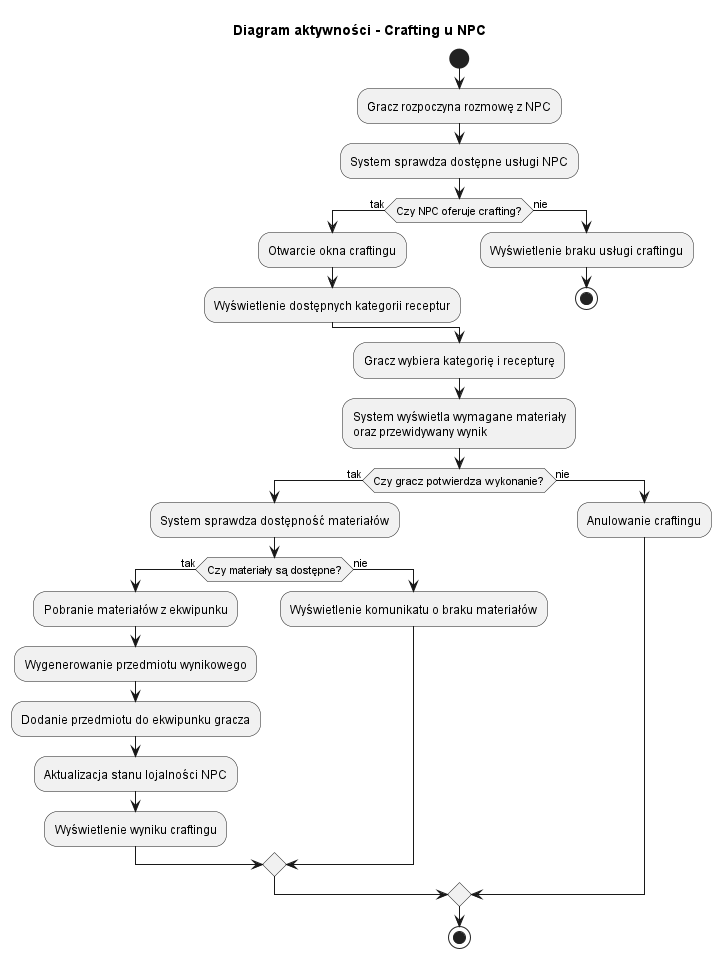
\includegraphics[width=\textwidth,height=0.72\textheight,keepaspectratio]{figures/uml/akt1.png}
    \caption{Diagram aktywności przedstawiający proces craftingu u NPC.}
    \label{fig:activity-crafting-npc}
    \wsizsource{Opracowanie własne}
\end{figure}

Diagram przedstawia przebieg procesu tworzenia przedmiotów z perspektywy gracza i systemu. Uwzględniono w nim zarówno weryfikację dostępności usługi craftingu u danego NPC, jak i sprawdzenie wymaganych materiałów przed wykonaniem operacji. Diagram pokazuje również możliwe ścieżki alternatywne, takie jak brak odpowiedniej usługi lub anulowanie procesu przez gracza.

\begin{figure}[H]
    \centering
    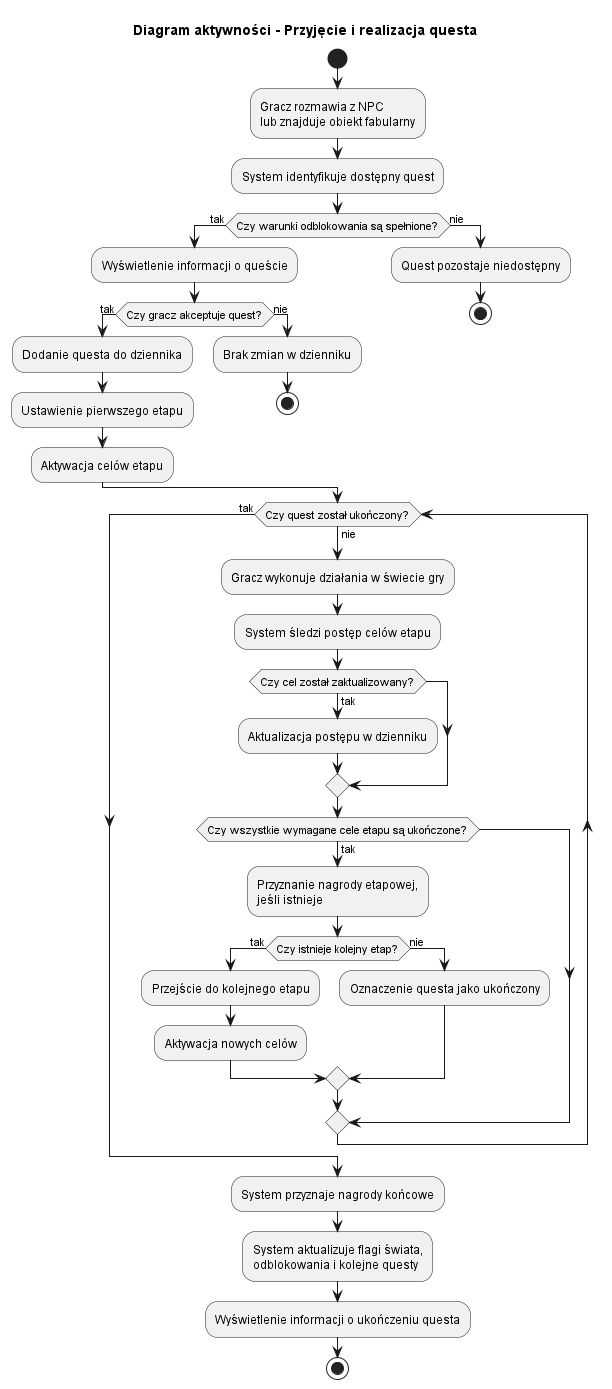
\includegraphics[width=\textwidth,height=0.72\textheight,keepaspectratio]{figures/uml/akt2.png}
    \caption{Diagram aktywności przedstawiający przyjęcie i realizację questa.}
    \label{fig:activity-quest-flow}
    \wsizsource{Opracowanie własne}
\end{figure}

Diagram opisuje pełny cykl życia zadania od momentu jego wykrycia do zakończenia i przyznania nagród. Pokazano na nim mechanizmy sprawdzania warunków odblokowania, akceptacji zadania przez gracza oraz aktualizacji postępu w kolejnych etapach. Ujęto także możliwość przechodzenia do następnych etapów oraz aktualizacji stanu świata po ukończeniu questa.

\subsection{Diagramy sekwencji}

\begin{figure}[H]
    \centering
    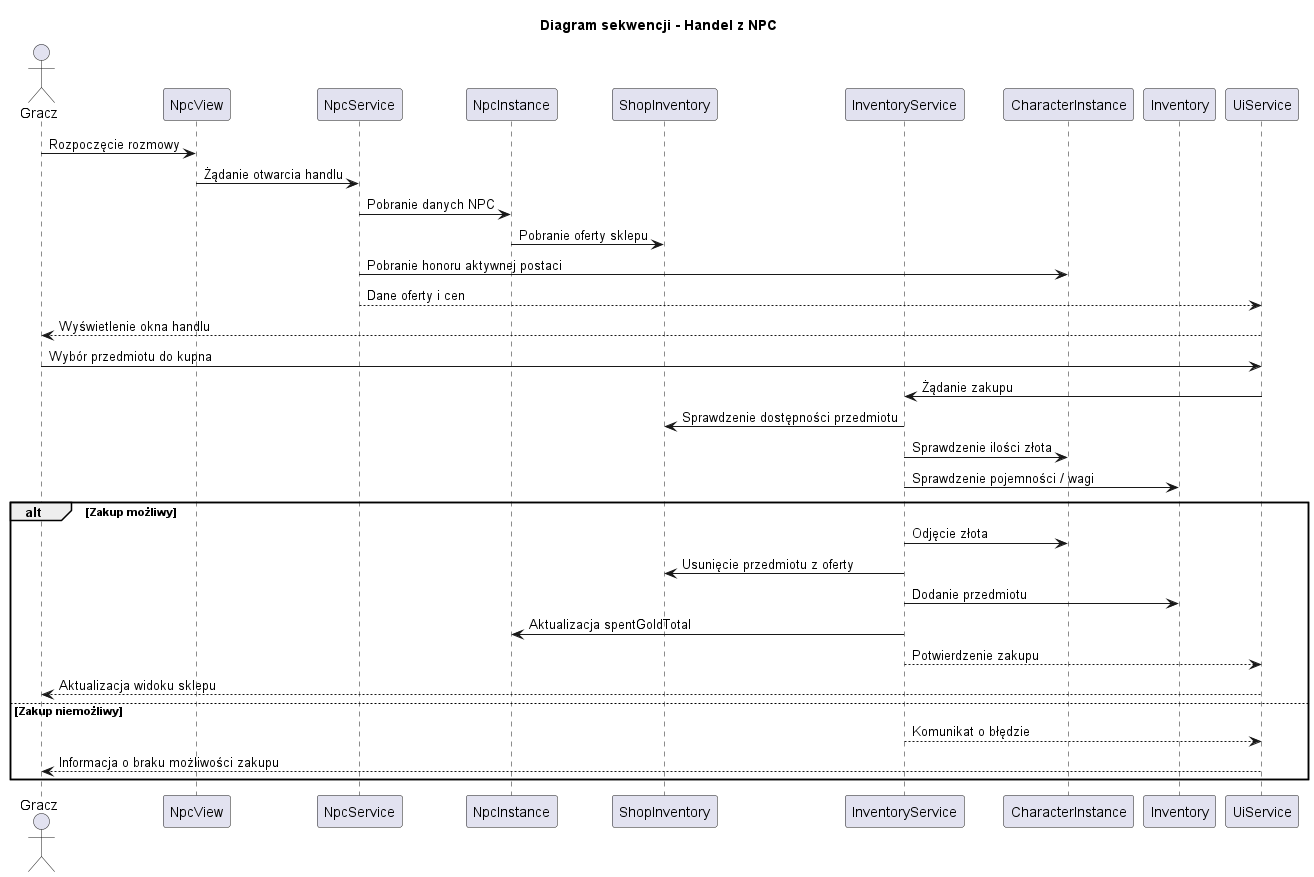
\includegraphics[width=\textwidth,height=0.72\textheight,keepaspectratio]{figures/uml/sek1.png}
    \caption{Diagram sekwencji przedstawiający handel z NPC.}
    \label{fig:sequence-trade-npc}
    \wsizsource{Opracowanie własne}
\end{figure}

Diagram sekwencji pokazuje współpracę pomiędzy interfejsem użytkownika, systemem NPC, ekwipunkiem oraz logiką zakupu podczas handlu. Proces rozpoczyna się od wejścia w interakcję z postacią niezależną i otwarcia okna handlu, a następnie przechodzi do weryfikacji oferty, ilości złota oraz ograniczeń ekwipunku. Diagram uwzględnia zarówno poprawny zakup, jak i sytuację, w której transakcja nie może zostać zrealizowana.

\begin{figure}[H]
    \centering
    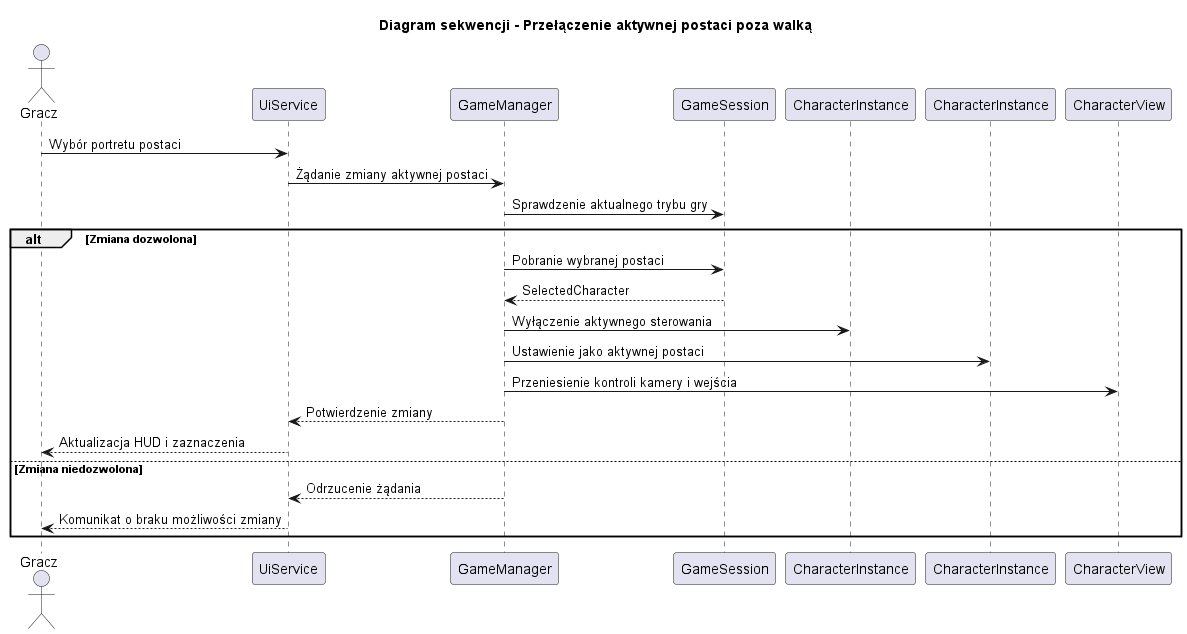
\includegraphics[width=\textwidth,height=0.72\textheight,keepaspectratio]{figures/uml/sek2.png}
    \caption{Diagram sekwencji przedstawiający przełączenie aktywnej postaci poza walką.}
    \label{fig:sequence-switch-active-character}
    \wsizsource{Opracowanie własne}
\end{figure}

Diagram obrazuje proces zmiany aktualnie sterowanej postaci w trybie eksploracji. Pokazano w nim sprawdzenie, czy zmiana jest dozwolona w bieżącym stanie gry, a następnie przekazanie sterowania nowo wybranej postaci oraz aktualizację warstwy prezentacji. Uwzględniono również ścieżkę alternatywną, w której zmiana zostaje odrzucona przez system.

\subsection{Diagramy stanów}

\begin{figure}[H]
    \centering
    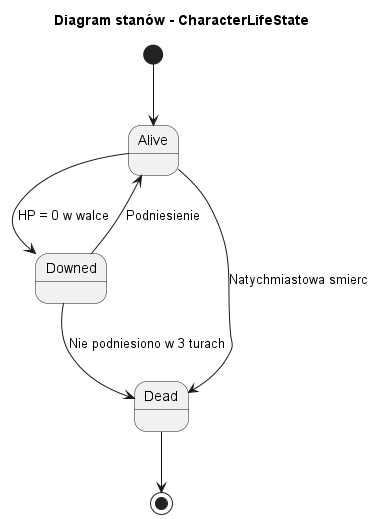
\includegraphics[width=0.75\textwidth,height=0.50\textheight,keepaspectratio]{figures/uml/stan1.png}
    \caption{Diagram stanów obiektu CharacterLifeState.}
    \label{fig:state-character-life}
    \wsizsource{Opracowanie własne}
\end{figure}

Diagram stanów przedstawia możliwe stany życia postaci oraz warunki przejścia pomiędzy nimi. Model obejmuje stan aktywny, powalenie oraz śmierć definitywną, zgodnie z założeniami systemu walki w grze. Szczególnie istotne jest tu przejście ze stanu \textit{Downed} do \textit{Dead}, które następuje, gdy postać nie zostanie podniesiona w ciągu trzech tur.

\begin{figure}[H]
    \centering
    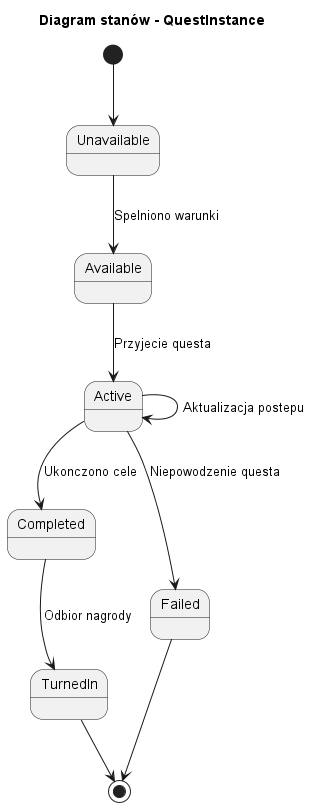
\includegraphics[width=0.82\textwidth,height=0.55\textheight,keepaspectratio]{figures/uml/stan2.png}
    \caption{Diagram stanów obiektu QuestInstance.}
    \label{fig:state-quest-instance}
    \wsizsource{Opracowanie własne}
\end{figure}

Diagram opisuje zmiany stanu instancji zadania w trakcie jego udostępniania, realizacji i zamykania. Uwzględniono w nim etap odblokowania zadania, jego przyjęcie, aktualizację postępu, ukończenie oraz odbiór nagrody. Model przewiduje również możliwość niepowodzenia zadania, co pozwala odwzorować bardziej złożone przebiegi misji w systemie questów.
\section{Technologie i wymagania sprzętowe}
\label{sec:technologie-i-wymagania}

Wybór technologii zastosowanych w projekcie \emph{Godmist} wynika z charakteru systemu oraz założonego zakresu funkcjonalnego. Projektowana aplikacja jest grą komputerową typu single player, łączącą eksplorację lochów, walkę turową, rozwój postaci, system przedmiotów, crafting, interakcje z NPC oraz trwały zapis postępu użytkownika. Oznacza to konieczność zastosowania narzędzi, które umożliwiają zarówno budowę warstwy wizualnej i interaktywnej, jak i czytelne modelowanie logiki systemu oraz trwałości danych.

W niniejszej sekcji przedstawiono główne technologie planowane do wykorzystania w projekcie oraz orientacyjne wymagania sprzętowe dla uruchomienia systemu. Ze względu na fakt, że projekt znajduje się na etapie dokumentacji i modelowania, część parametrów technicznych ma charakter założeń wstępnych i może zostać doprecyzowana na dalszych etapach implementacji.

\subsection{Technologie}
\label{subsec:technologie}

Podstawową technologią zastosowaną w projekcie jest silnik \emph{Unity}. Został on wybrany ze względu na szerokie możliwości tworzenia gier 2D, dobrą integrację warstwy wizualnej z logiką systemu oraz wygodny model pracy oparty na scenach, komponentach i obiektach. Unity umożliwia również stosowanie wzorców architektonicznych wspierających rozdzielenie definicji danych, logiki runtime oraz warstwy prezentacji, co jest istotne z punktu widzenia utrzymania porządku w projekcie.

Językiem implementacji systemu jest \emph{C\#}. Wybór ten wynika bezpośrednio z integracji z silnikiem Unity, ale również z cech samego języka, takich jak obiektowy model programowania, dobra organizacja kodu, możliwość modelowania złożonych struktur danych oraz wygodne tworzenie klas domenowych, serwisów i warstw pośrednich. W projekcie zakłada się szerokie wykorzystanie klas reprezentujących zarówno definicje danych, jak i zmienny stan rozgrywki.

Ważnym elementem architektury systemu jest wykorzystanie obiektów \texttt{ScriptableObject}. Mechanizm ten pozwala przechowywać definicje statycznych danych gry, takich jak klasy postaci, definicje przedmiotów, umiejętności, questy czy definicje lochów. Dzięki temu możliwe jest oddzielenie danych konfiguracyjnych od runtime'owego stanu gry oraz łatwiejsze rozwijanie projektu bez konieczności wprowadzania wszystkich zmian bezpośrednio w kodzie źródłowym.

Do przechowywania stanu gry planowane jest zastosowanie plików \emph{JSON}. Rozwiązanie to jest odpowiednie dla gry single player, w której nie ma potrzeby wykorzystywania zewnętrznej, relacyjnej bazy danych. Zapis w formacie JSON umożliwia przechowywanie stanu postaci, misji, NPC, lochów, ekwipunku i innych elementów w sposób strukturalny i łatwy do odtworzenia. Model ten dobrze współgra z projektowaną architekturą opartą na identyfikatorach definicji i klasach runtime.

W procesie projektowania wykorzystywane są również diagramy UML oraz narzędzia do modelowania wizualnego. Ich zadaniem jest uporządkowanie struktury systemu i przedstawienie zależności pomiędzy jego elementami jeszcze przed pełną implementacją. Dzięki temu możliwe jest wczesne wykrywanie niespójności oraz bardziej świadome planowanie podziału systemu na moduły.

Można zatem przyjąć, że główny stos technologiczny projektu obejmuje:
\begin{itemize}
    \item silnik \emph{Unity},
    \item język programowania \emph{C\#},
    \item definicje danych oparte na \texttt{ScriptableObject},
    \item zapis stanu gry w plikach \emph{JSON},
    \item modelowanie projektowe z użyciem diagramów UML.
\end{itemize}

\subsection{Wymagania sprzętowe}
\label{subsec:wymagania-sprzetowe}

Projektowany system przeznaczony jest do uruchamiania na komputerach osobistych. Ze względu na charakter gry 2D oraz brak rozbudowanych wymagań związanych z renderingiem trójwymiarowym, nie przewiduje się bardzo wysokich wymagań sprzętowych. Jednocześnie system powinien działać stabilnie przy obsłudze walk wieloobiektowych, stanu drużyny, ekwipunku, lochów proceduralnych oraz mechanizmu zapisu i odczytu danych.

Na obecnym etapie projektu można przyjąć orientacyjne wymagania minimalne:
\begin{itemize}
    \item system operacyjny: Windows 10 lub nowszy,
    \item procesor: 64-bitowy, dwurdzeniowy,
    \item pamięć RAM: 8 GB,
    \item karta graficzna: zgodna z DirectX 11,
    \item wolne miejsce na dysku: co najmniej 2 GB.
\end{itemize}

Orientacyjne wymagania zalecane można określić następująco:
\begin{itemize}
    \item system operacyjny: Windows 10 lub nowszy,
    \item procesor: 64-bitowy, czterordzeniowy,
    \item pamięć RAM: 16 GB,
    \item karta graficzna: dedykowana karta obsługująca DirectX 11 lub nowszy,
    \item wolne miejsce na dysku: 4 GB lub więcej.
\end{itemize}

Wymagania te mają charakter wstępny i mogą ulec zmianie w zależności od ostatecznego zakresu implementacji, liczby zasobów graficznych, rozbudowy GUI oraz stopnia złożoności finalnych mechanik. Na obecnym etapie stanowią one jednak wystarczającą podstawę do określenia docelowej platformy działania systemu.

\section{Struktura systemu}
\label{sec:struktura-systemu}

Struktura systemu \emph{Godmist} została zaprojektowana w sposób warstwowy i modularny. Jest to szczególnie istotne ze względu na złożoność projektowanej gry, która łączy wiele współdziałających podsystemów, takich jak eksploracja lochów, walka turowa, rozwój postaci, ekwipunek, crafting, interakcje z NPC, system misji oraz trwałość stanu gry. Przyjęta organizacja rozwiązania ma umożliwiać nie tylko poprawne działanie systemu, ale również jego późniejszą rozbudowę i utrzymanie.

Projekt nie opiera się na klasycznej architekturze bazodanowej charakterystycznej dla systemów biznesowych lub aplikacji sieciowych. Zamiast tego wykorzystuje strukturę danych dopasowaną do gry single player, w której istotną rolę odgrywają definicje statyczne, zmienny stan runtime oraz zapis trwały odtwarzany pomiędzy sesjami użytkownika. Oznacza to konieczność rozdzielenia tych trzech poziomów odpowiedzialności i opisania ich w sposób uporządkowany.

\subsection{Opis modelu danych i trwałości}
\label{subsec:opis-modelu-danych}

W projekcie \emph{Godmist} przyjęto model danych oparty na rozdzieleniu definicji systemowych od danych runtime oraz trwałego zapisu stanu gry. Takie podejście pozwala uniknąć mieszania danych statycznych, które definiują reguły świata gry, z danymi zmiennymi, które opisują bieżący stan rozgrywki konkretnego użytkownika.

Pierwszą warstwę stanowią definicje statyczne. Są to dane opisujące elementy gry, które nie zmieniają się dynamicznie w ramach jednej kampanii, lecz pełnią rolę wzorców wykorzystywanych przez system. Do tej grupy należą między innymi definicje postaci, klas postaci, umiejętności, przedmiotów, NPC, questów i lochów. W architekturze projektu dane tego typu są reprezentowane jako obiekty \texttt{ScriptableObject}, co pozwala na ich czytelną organizację i łatwe rozwijanie w środowisku Unity.

Drugą warstwę stanowią dane runtime, czyli bieżący stan gry podczas działania aplikacji. Warstwa ta obejmuje między innymi stan postaci, aktywne questy, stan lochu, ekwipunek, relacje między drużynami w walce, efekty pasywne oraz aktualne położenie i stan obiektów świata. Dane te są modyfikowane w trakcie rozgrywki i odzwierciedlają aktualną sytuację użytkownika.

Trzecią warstwę stanowi trwałość danych, czyli sposób zapisu i odtwarzania stanu gry pomiędzy sesjami. W projekcie nie zastosowano klasycznej relacyjnej bazy danych. Zamiast tego zapis realizowany jest z wykorzystaniem plików \emph{JSON}. Rozwiązanie to jest uzasadnione charakterem gry single player, brakiem konieczności komunikacji z centralnym serwerem oraz potrzebą wygodnego odtwarzania rozbudowanego stanu gry. W zapisie przechowywane są między innymi dane postaci, stany przedmiotów, questów, NPC, lochów, schowka i świata.

Istotnym założeniem modelu danych jest identyfikowanie obiektów logicznych za pomocą stabilnych identyfikatorów tekstowych. Dzięki temu możliwe jest odwoływanie się do definicji danych oraz rekonstrukcja zależności pomiędzy obiektami podczas wczytywania gry. Przykładowo postać może odnosić się do definicji swojej klasy, przedmiot do definicji typu przedmiotu, a quest do definicji etapu lub celu. Takie podejście upraszcza serializację danych i wspiera modularny charakter projektu.

W przypadku lochów proceduralnych zastosowano podejście oparte na przechowywaniu ziarna generowania oraz zmian względem stanu bazowego. Oznacza to, że zamiast zapisywania pełnej, surowej kopii każdego elementu runtime, system może odtwarzać strukturę lochu na podstawie parametrów generacji i zapamiętanych różnic, takich jak odwiedzone pomieszczenia, pokonane walki czy aktywowane obiekty. Pozwala to ograniczyć złożoność zapisu i lepiej dopasować model trwałości do charakteru gry.

\subsection{Diagram ERD}
\label{subsec:diagram-erd}

\begin{figure}[H]
    \centering
    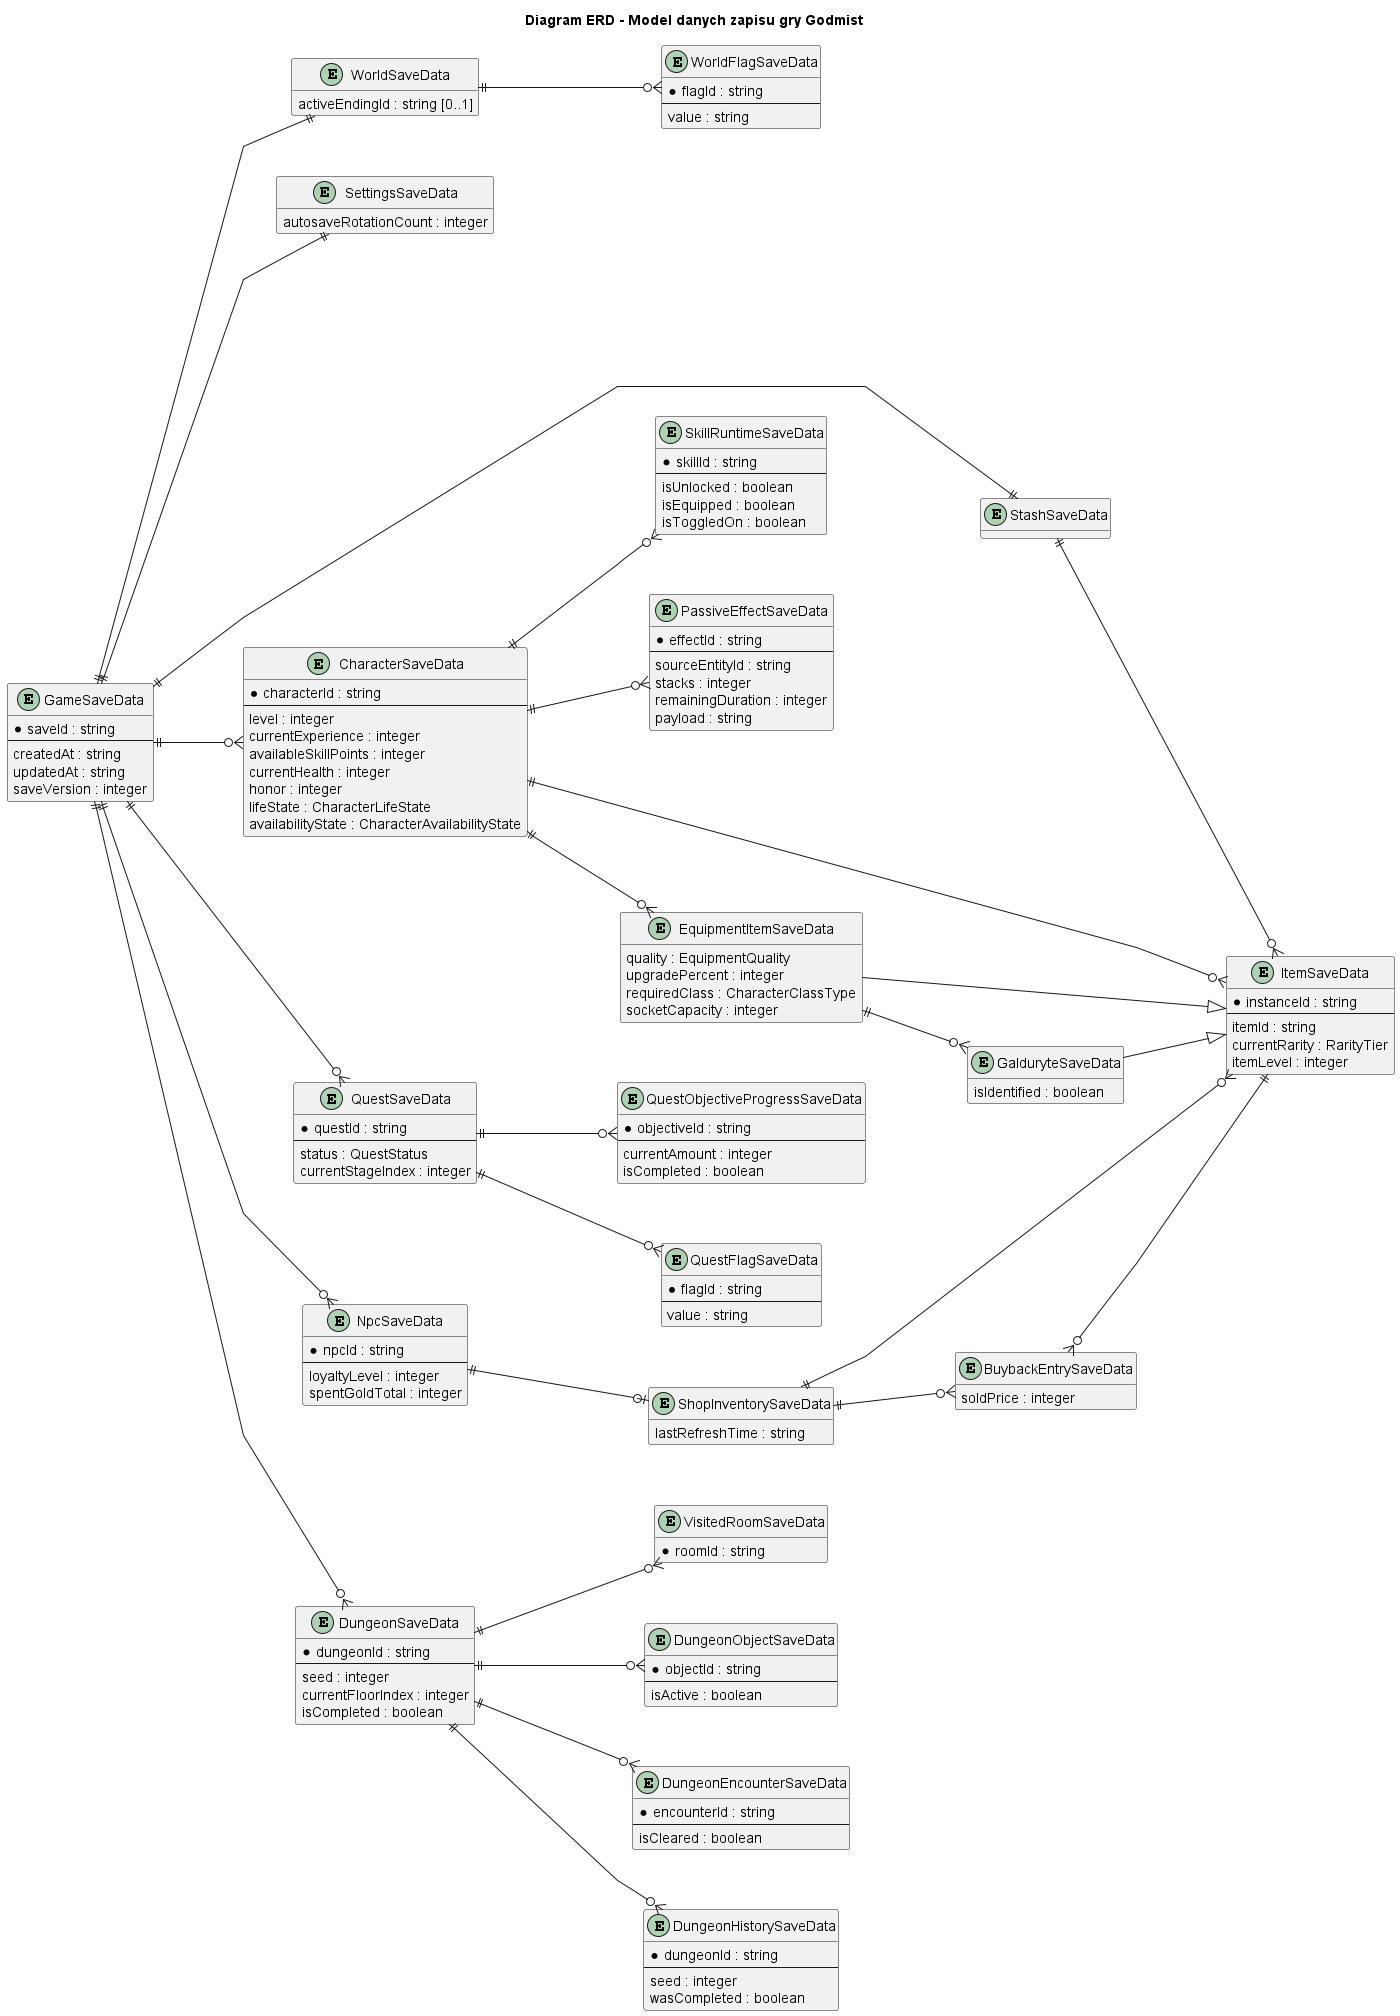
\includegraphics[width=\textwidth,height=0.82\textheight,keepaspectratio]{figures/uml/erd.png}
    \caption{Diagram ERD logicznego modelu danych zapisu gry Godmist.}
    \label{fig:erd-godmist}
    \wsizsource{Opracowanie własne}
\end{figure}

Ze względu na charakter projektowanego systemu diagram ERD nie przedstawia klasycznej relacyjnej bazy danych, lecz logiczny model encji i zależności wykorzystywanych do zapisu stanu gry. Ujęto na nim najważniejsze struktury trwałe, takie jak zapis globalny, stan świata, postacie, questy, NPC, lochy oraz dane związane z przedmiotami i schowkiem. Diagram pokazuje również relacje właścicielskie pomiędzy głównym obiektem zapisu a jego elementami składowymi, a także zależności pomiędzy specjalizacjami danych przedmiotów. Taka forma modelu danych lepiej odpowiada architekturze gry single player wykorzystującej pliki JSON niż klasyczny schemat tabel relacyjnych.

\subsection{Diagram klas}
\label{subsec:diagram-klas}

\begin{figure}[H]
    \centering
    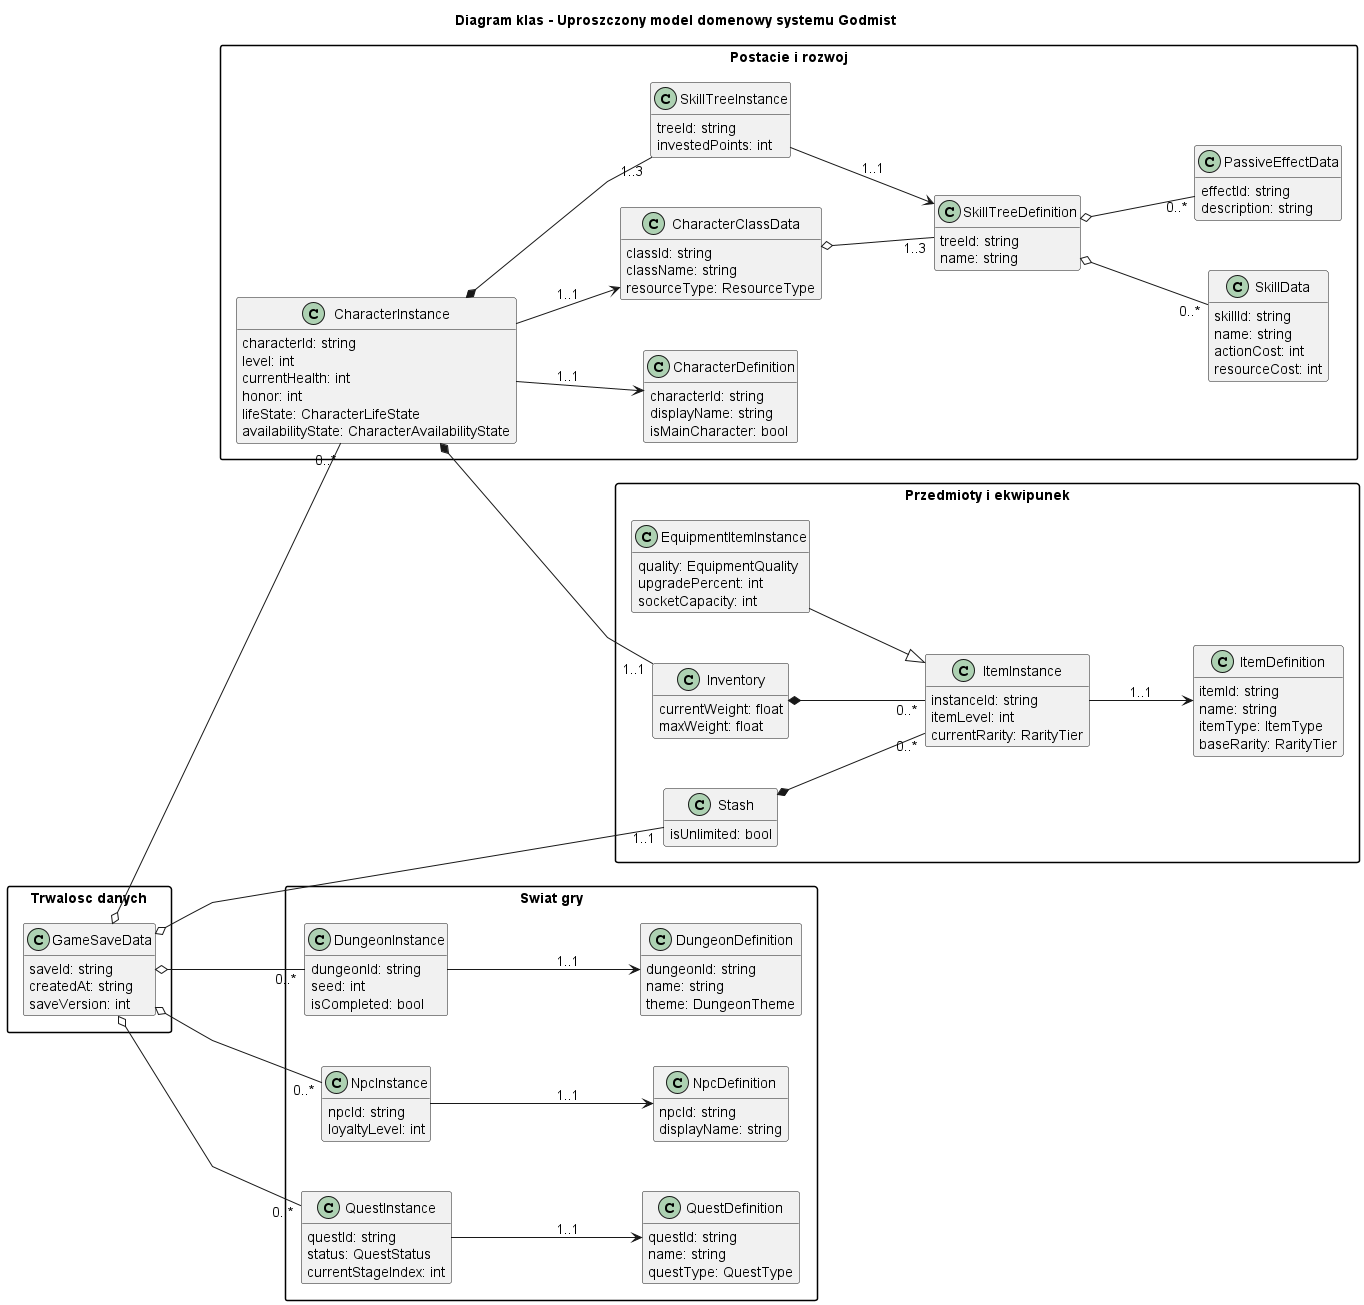
\includegraphics[width=\textwidth,height=0.82\textheight,keepaspectratio]{figures/uml/class-diagram.png}
    \caption{Uproszczony diagram klas systemu Godmist.}
    \label{fig:class-diagram-godmist}
    \wsizsource{Opracowanie własne}
\end{figure}

Na potrzeby niniejszej dokumentacji przedstawiono uproszczony diagram klas, którego celem jest pokazanie najważniejszych klas domenowych systemu oraz zależności pomiędzy nimi. Diagram nie stanowi pełnego odwzorowania wszystkich klas projektowych i implementacyjnych, lecz syntetyczny model obejmujący kluczowe obszary systemu: postacie i rozwój, przedmioty i ekwipunek, świat gry oraz trwałość danych. Takie uproszczenie zostało zastosowane celowo, aby zachować czytelność modelu i umożliwić jego analizę na poziomie architektury logicznej systemu.

Na diagramie widoczne są zależności pomiędzy definicjami danych, instancjami runtime oraz głównym obiektem zapisu gry. Pokazano między innymi relacje pomiędzy definicją postaci a jej instancją, powiązania klas postaci z drzewkami rozwoju, zależności pomiędzy instancjami przedmiotów i ich definicjami, a także relacje łączące zapis gry ze stanem postaci, questów, NPC, lochu i schowka. Dzięki temu diagram stanowi podsumowanie struktury domenowej systemu i uzupełnia wcześniejsze modele zachowania oraz model danych trwałych przedstawiony na diagramie ERD.

Warto podkreślić, że na diagramie pominięto część klas pomocniczych i szczegółowych mechanizmów, takich jak klasy widoku, serwisy systemowe, szczegółowe klasy walki, niższopoziomowe struktury zapisu oraz wybrane obiekty pomocnicze związane z mechanikami specjalistycznymi. Zabieg ten pozwolił skupić się na relacjach najistotniejszych z perspektywy projektowej i inżynierskiej. W efekcie diagram klas pełni w pracy rolę modelu poglądowego, porządkującego logikę architektury systemu, a nie pełnej dokumentacji implementacyjnej wszystkich elementów projektu.

\subsection{Architektura warstwowa systemu}
\label{subsec:architektura-warstwowa}

Projekt \emph{Godmist} wykorzystuje architekturę warstwową, której celem jest rozdzielenie odpowiedzialności pomiędzy definicje danych, logikę domenową, serwisy systemowe oraz warstwę prezentacji. Takie podejście jest szczególnie korzystne w środowisku Unity, ponieważ pozwala ograniczyć nadmierne mieszanie logiki gry z klasami odpowiedzialnymi za scenę, widok i wejście użytkownika.

Pierwszą warstwę stanowią definicje danych. Obejmuje ona obiekty \texttt{ScriptableObject}, które przechowują statyczne informacje o klasach postaci, umiejętnościach, questach, przedmiotach, NPC i lochach. Warstwa ta pełni funkcję konfiguracji systemu i nie reprezentuje bezpośrednio zmiennego stanu rozgrywki.

Drugą warstwę stanowi model domenowy runtime. W jej skład wchodzą klasy reprezentujące aktualny stan postaci, walki, lochu, NPC, questów oraz innych elementów rozgrywki. To właśnie ta warstwa odpowiada za odwzorowanie bieżącej sytuacji w grze i przechowuje dane, które ulegają zmianom w trakcie działania aplikacji.

Trzecią warstwę tworzą serwisy systemowe. Ich zadaniem jest koordynowanie działania poszczególnych obszarów funkcjonalnych, takich jak walka, eksploracja, questy, inventory, crafting, NPC czy zapis gry. Serwisy te nie pełnią roli widoków ani definicji danych, lecz realizują logikę operacyjną i pośredniczą pomiędzy stanem gry a interakcjami użytkownika.

Czwartą warstwę stanowi warstwa prezentacji. Obejmuje ona klasy \texttt{MonoBehaviour}, które odpowiadają za wyświetlanie obiektów na scenie, obsługę interakcji użytkownika, integrację z UI oraz reagowanie na zmiany stanu systemu. W tej warstwie mieszczą się między innymi widoki postaci, NPC, obiektów lochu i okien interfejsu użytkownika.

Uzupełnieniem całej architektury jest warstwa trwałości danych, odpowiedzialna za serializację i deserializację stanu gry. Obejmuje ona klasy DTO wykorzystywane do zapisu w formacie JSON oraz komponenty odpowiedzialne za koordynację operacji zapisu i odczytu. Dzięki temu model definicji, runtime i trwałości pozostaje rozdzielony, co poprawia czytelność rozwiązania i ogranicza ryzyko niekontrolowanego przenikania się odpowiedzialności pomiędzy modułami.

Przyjęty podział warstwowy wspiera dalszy rozwój projektu, ponieważ umożliwia niezależną rozbudowę poszczególnych obszarów systemu. Pozwala również łatwiej identyfikować zależności pomiędzy elementami rozwiązania oraz zachować większą kontrolę nad architekturą w miarę wzrostu złożoności gry.

\section{Podsumowanie rozdziału}
\label{sec:podsumowanie-rozdzialu-2}

W niniejszym rozdziale przedstawiono projekt systemu \emph{Godmist} z perspektywy modelowania, doboru technologii oraz organizacji struktury rozwiązania. Omówiono rolę modeli UML jako narzędzia służącego do opisu zachowania i struktury systemu, wskazano główne technologie planowane do wykorzystania w projekcie oraz scharakteryzowano sposób organizacji danych i trwałości stanu gry.

Szczególną uwagę zwrócono na fakt, że projekt nie wykorzystuje klasycznej relacyjnej bazy danych, lecz opiera się na rozdzieleniu definicji statycznych, stanu runtime oraz zapisu trwałego realizowanego z użyciem plików JSON. Pozwoliło to przedstawić architekturę rozwiązania w sposób lepiej dopasowany do charakteru gry single player oraz do przyjętych założeń technologicznych.

Przedstawiona struktura systemu stanowi podstawę do dalszego opisu bardziej praktycznych aspektów projektu. W kolejnym rozdziale omówiony zostanie interfejs użytkownika, propozycje testów oraz końcowe wnioski dotyczące projektowanego rozwiązania.
